%%%%%%%%%%%%%%%%%%%%%%%%%%%%%%%%%%%%%%%%%%%%%%%%%%%%%%%%%%%%%%%%%%%%%%%%%%%%%%%%
%2345678901234567890123456789012345678901234567890123456789012345678901234567890
%        1         2         3         4         5         6         7         8

%\documentclass[journal,transmag]{IEEEtran}% Comment this line out if you need a4paper

\documentclass[10pt, conference]{ieeeconf}      % Use this line for a4 paper

\IEEEoverridecommandlockouts                              % This command is only needed if 
                                                          % you want to use the \thanks command

%\overrideIEEEmargins                                      % Needed to meet printer requirements.

% See the \addtolength command later in the file to balance the column lengths
% on the last page of the document

% The following packages can be found on http:\\www.ctan.org
%\usepackage{graphics} % for pdf, bitmapped graphics files
%\usepackage{epsfig} % for postscript graphics files
%\usepackage{mathptmx} % assumes new font selection scheme installed
%\usepackage{times} % assumes new font selection scheme installed
%\usepackage{amsmath} % assumes amsmath package installed
%\usepackage{amssymb}  % assumes amsmath package installed

\newtheorem{theorem}{Theorem}[section]
\newtheorem{lemma}[theorem]{Lemma}
\newtheorem{proposition}[theorem]{Proposition}
\newtheorem{corollary}[theorem]{Corollary}
\usepackage[ruled,vlined]{algorithm2e}

\newcommand{\qed}{\nobreak \ifvmode \relax \else
      \ifdim\lastskip<1.5em \hskip-\lastskip
      \hskip1.5em plus0em minus0.5em \fi \nobreak
      \vrule height0.75em width0.5em depth0.25em\fi}

\def\lc{\left\lfloor}   
\def\rc{\right\rfloor}

\usepackage{amsmath,amssymb}

\usepackage{tabularx}
\usepackage{tikz,hyperref,graphicx,units}
\usepackage{subfigure}
\usepackage{benktools}

\usepackage{caption}
\usepackage{epstopdf}
\renewcommand{\captionfont}{\footnotesize}
\usepackage{sidecap,wrapfig}
\usepackage[ruled,vlined]{algorithm2e}
\DeclareMathOperator*{\argmin}{arg\,min}
\DeclareMathOperator*{\argmax}{arg\,max}
\newcommand{\abs}[1]{\lvert#1\rvert} 
\newcommand{\norm}[1]{\lVert#1\rVert}
%\newcommand{\suchthat}{\mid}
\newcommand{\suchthat}{\ \big|\ }
\newcommand{\ba}{\mathbf{a}}
\newcommand{\bb}{\mathbf{b}}
\newcommand{\bc}{\mathbf{c}}
\newcommand{\bd}{\mathbf{d}}
\newcommand{\bg}{\mathbf{g}}
\newcommand{\bj}{\mathbf{j}}
\newcommand{\bn}{\mathbf{n}}
\newcommand{\bp}{\mathbf{p}}
\newcommand{\bw}{\mathbf{w}}
\newcommand{\bt}{\mathbf{t}}
\newcommand{\bu}{\mathbf{u}}
\newcommand{\by}{\mathbf{y}}
\newcommand{\bx}{\mathbf{x}}
\newcommand{\bz}{\mathbf{z}}
\newcommand{\bbf}{\mathbf{f}}
\newcommand{\bzero}{\mathbf{0}}
\newcommand{\bG}{\mathbf{G}}
\newcommand{\bA}{\mathbf{A}}
\newcommand{\bW}{\mathbf{W}}
\newcommand{\bX}{\mathbf{X}}
\newcommand{\mX}{\mathcal{X}}
\newcommand{\mD}{\mathcal{D}}
\newcommand{\mG}{\mathcal{G}}
\newcommand{\mN}{\mathcal{N}}
\newcommand{\mW}{\mathcal{W}}
\newcommand{\mF}{\mathcal{F}}
\newcommand{\bZ}{\mathbf{Z}}
\newcommand{\mR}{\mathcal{R}}

\newcommand{\bfc}{W}
\newcommand{\Qinf}{Q_{\infty}}
\newcommand{\st}[1]{_\text{#1}}
\newcommand{\rres}{r\st{res}}
\newcommand{\pos}[1]{(#1)^+}
\newcommand{\depth}{\operatorname{depth}}
\newcommand{\dist}{\operatorname{dist}}
\newcommand{\convhull}{\operatorname{ConvexHull}}
\newcommand{\minksum}{\operatorname{MinkowskiSum}}

\newcommand{\specialcell}[2][c]{ \begin{tabular}[#1]{@{}c@{}}#2\end{tabular}}
\newcommand{\acro}{SHIV}
\newcommand\independent{\protect\mathpalette{\protect\independenT}{\perp}}
\def\independenT#1#2{\mathrel{\rlap{$#1#2$}\mkern2mu{#1#2}}}

\newcolumntype{L}[1]{>{\RaggedRight\hspace{0pt}}p{#1}}
\newcolumntype{R}[1]{>{\RaggedLeft\hspace{0pt}}p{#1}}

\title{\LARGE \bf \acro: Reducing Supervisor Burden using SVM-based Risk to Efficiently Learn Robot Control Policies
from Demonstrations {\color{blue}(v.10)} }

\author{Michael Laskey$^1$,Wesley Yu-Shu Hsieh, Jeff Mahler, Florian T. Pokorny$^1$, Ken Goldberg$^2$% <-this % stops a space
\thanks{$^1$Department of Electrical Engineering and Computer Sciences; {\small \{mdlaskey, ftpokorny\}@berkeley.edu}}%
\thanks{$^2$Department of Industrial Engineering and Operations Research and Department of Electrical Engineering and Computer Sciences; {\small goldberg@berkeley.edu}}%
\thanks{$^{1-2}$ University of California, Berkeley;  Berkeley, CA 94720, USA}%
} 

\begin{document}



\maketitle
\thispagestyle{empty}
\pagestyle{empty}


%%%%%%%%%%%%%%%%%%%%%%%%%%%%%%%%%%%%%%%%%%%%%%%%%%%%%%%%%%%%%%%%%%%%%%%%%%%%%%%%

\begin{abstract}
For robot control problems where no reward function is known and the dynamics of the environment are not specified, the
learning from demonstrations approach provides an algorithmic paradigm for learning a policy from supervisor-provided
demonstrations. Dataset Aggregation (DAgger) in particular yields a state of the art method in this context which treats
the problem of determining a policy as an iterative supervised learning problem. DAgger alternates between executing a
trained policy and acquiring new supervisor control inputs for roll-outs of a current best policy estimator. 
We propose a novel algorithm, \acro~ based on DAgger which estimates the riskiness of states
encountered by the policy roll-outs by means of an approximate quantile super-levelset estimate of the distribution of
states used for training the current policy and which additionally takes empirical surrogate loss of the current policy
into account. Since learning a quantile function for high-dimensional input data is
challenging, we instead modify an SVN-based approach to quantile estimation that employs regularization to solve this
problem approximately. Our algorithm considers roll-outs with early termination as soon as a state outside a
user-defined quantile super-levelset is encountered. Our approach empirically reduces the amount of neccessary
supervisor demonstrations by only collecting supervisor control inputs at states outside the current quantile estimate.
In experiments involving a simulated race track and in a Super Mario Atari game benchmark considered by the authors of
DAgger, our approach results in similar peak performance levels as DAgger while reducing the amount of required supervisor
control inputs by more than {\color{blue}[-- TODO --]} percent.
\end{abstract}


%%%%%%%%%%%%%%%%%%%%%%%%%%%%%%%%%%%%%%%%%%%%%%%%%%%%%%%%%%%%%%%%%%%%%%%%%%%%%%%%

\section{Introduction} 
Consider the problem of teaching a robot a complex task such cooking a meal or racing a toy car around a track
against human opponents. When the robot is only provided with visual demonstrations without the knowledge or an
underlying cost function describing the task, traditional model-based control approaches are often not applicable. In
these situations, the learning from demonstrations (LfD) approach provides a paradigmn for teaching the robot how to
accomplish the task \cite{ross2013learning,pomerleau1989alvinn,schulman2013case}.

One approach to LfD is to train a policy, or a function estimator (either a classifier or regressor), to predict a
supervisor's behavior given training data consisting of pairs of observations (input) and control inputs (output) performed
while accomplishing a task. Since the robot's actions typically affect the resulting next state, the resulting sequences
of states encountered during the execution of a policy are not independent random variables, thus making statistical
inference challenging. Ross et al. proved that this can cause the error in the policy estimator to compound over 
time and lead to performance degradation that is proportional to the time horizon of the task squared. The intuition
behind this result is that as the robot makes mistakes with respect to the supervisor's policy it drifts from the
distribution it was trained on and might encounter new states it can't generalize to.  Ross and Bagnell overcome this by
presenting an iterative method that first trains a policy on the data observed using standard supervised learning
techniques and then tries (or 'rolls out') the policy in the environment to see what states are likely to occur under
the robot's trained policy.  The supervisor then tells the robot what controls it should have applied after each iteration
and the policy is retrained \cite{ross2010reduction}. The DAgger method has been successfully used since to teach a
robot how to follow verbal instructions, achieve state of the art performance on Atari games and fly a quad copter
through a forest~\cite{NIPS2014_5421,duvallet2013imitation,ross2013learning}.




\begin{figure}[t!]
\centering
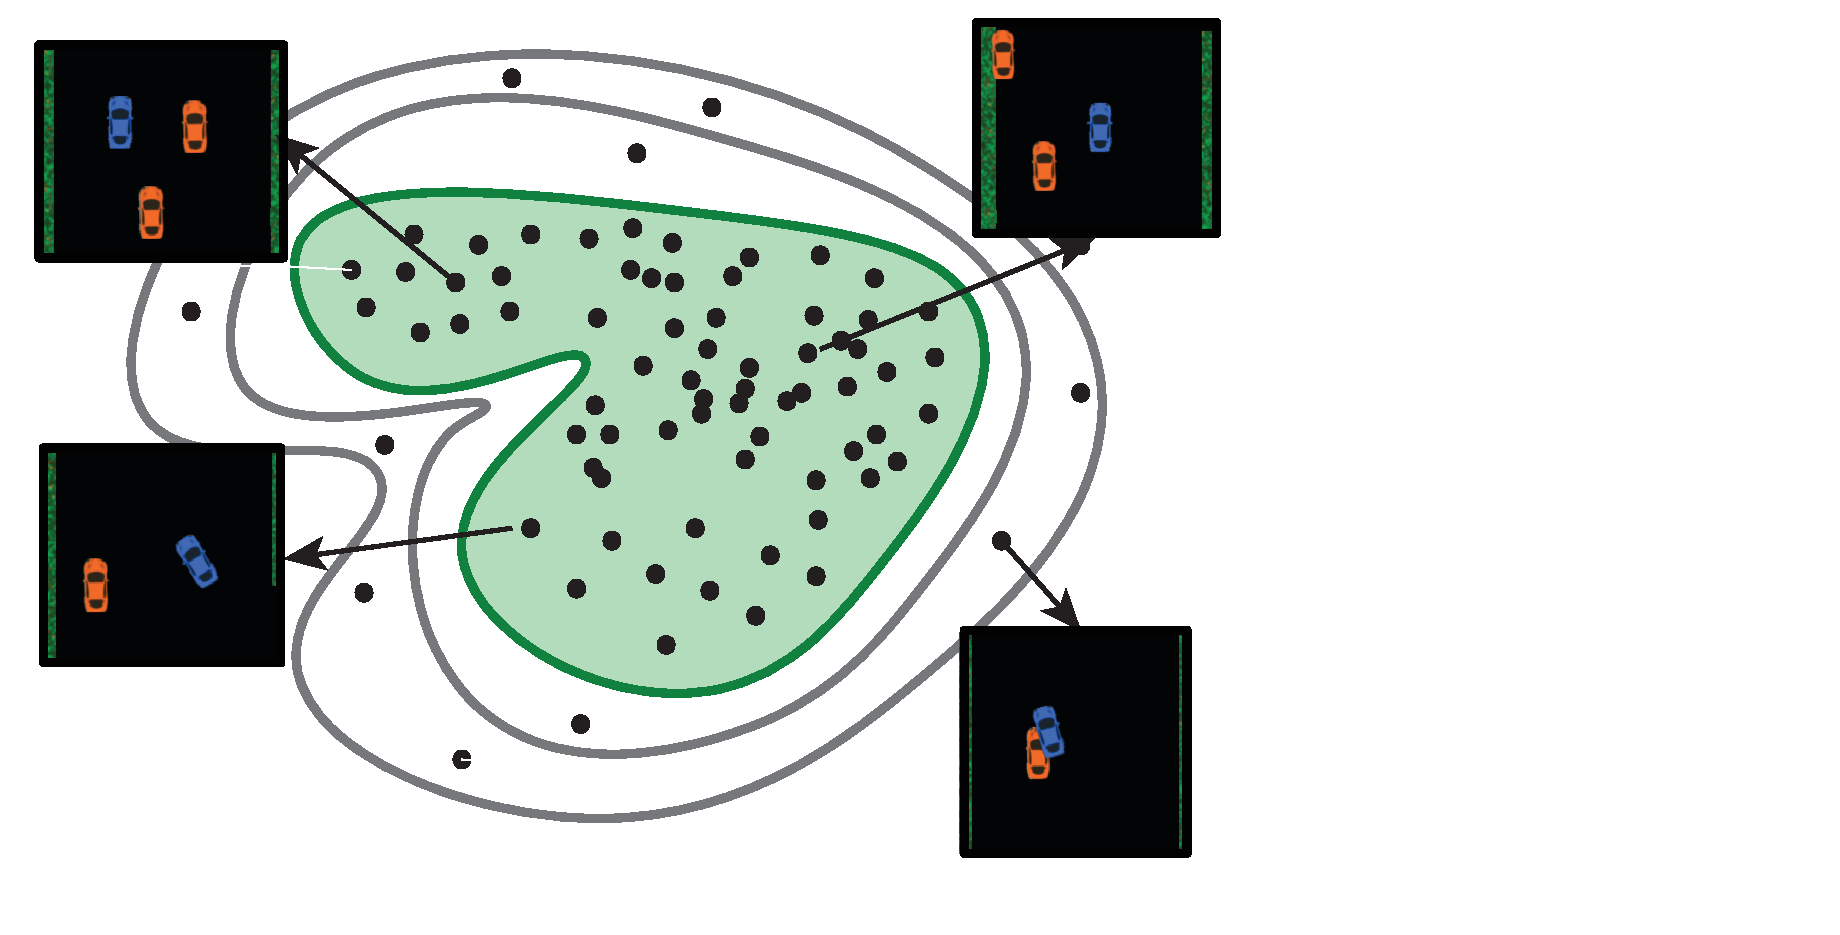
\includegraphics[width=12cm, height=6cm]{figures/teaser.eps}
\caption{ 
Given a set of states corresponding to images of a race-track simulation (visualized in $\mathbb{R}^2$) with expert
control inputs, we consider a modified quantile super-levelset estimate (shaded) as an approximation of the riskiness of
executing the trained policy at a given state. By varying the quantile threshold, we can increase or decrease the size
of the quantile super-levelset area. In our approach, points outside the super-levelset are considered risky and, during
training, roll-outs of the policy that leave the super-levelset require control input demonstrations from the supervisor,
while roll-outs within the super-levelset can be performed autonomously.
}
\vspace*{-10pt}
\label{fig:dis_traveled}
\end{figure}

During learning, implementations of DAgger require the supervisor to manually provide control inputs that the robot
should have applied for each states it visits when rolling out the current best policy estimate. If the supervisor is a
human or an algorithm with a high time complexity, this can be tedious or expensive. We are hence interested in
reducing the burdon on the supervisor by partitioning the state space into states where the policy can either be
executed autonomously with little expected risk, or where supervisor control input (or 'labels') are likely to be
required due to high risk. We postulate that a state can be risky for 2 reasons: 1) we encounter a state which has a low density of
training data in its vicinity, which potentially means our policy will mis-predict the supervisor
\cite{tokdar2010importance} 2) the state is potentially near previously visited states, but the control-input is mis-predicted
nonetheless. If an accurate density estimation corresponding to
the pairs of visited states and control signals is available, the first scenario can be captured by regions of
state-space with a low density estimate. Areas of low density are then considered to be risky since insufficient data
is available to accurately model the demonstrator's policy. This idea is also captured in the notion that 'a trained
model will be able to generalize within the distribution it is trained on' \cite{tokdar2010importance} in statistical
machine learning. The second case arises for example when the current best policy estimate is locally inconsistent with expert
demonstrations.
%
%Vague!!!
%This property can be seen used in importance sampling when data is collected from one distribution, but tested on
%another and has to be re-weighted %to the test distribution \cite{huang2006correcting}. 
%
While the amount of data needed to accurately estimate the density increases exponentially with the dimension of state
space \cite{nadaraya1964estimating}, we can turn to approximate methods which instead attempt to learn an approximate
representation of the quantile levelsets of the distribution. Thus, we propose using a modified version the One Class
SVM method for support estimation that only tries to estimate the level set of the quantile function of the density
\cite{scholkopf2001estimating} at a user-determined quantile threshold which has been used even with high-dimensional
image data \cite{liu2014unsupervised}. Our modification furthermore removes areas of state space from the super-levelset
estimate where the local policy estimate is inconsistent with the expert demonstrations in the sense that the incurred
surrogate loss of the current policy relative to the expert demonstration is above a threshold $\varepsilon>0$.

To apply our approach, we make the same basic assumptions as DAgger: 1) we require access to an environment
where a robot can try out (roll out) policies to sample trajectories and where we are able to collect observation states
and corresponding control inputs along these trajectories. 2) an interface allowing a supervisor to provide control
inputs that should have been applied for states along parts of the rolled out trajectories. 3) We assume that we are
able to collect a series of observations from the environment and the controls applied. 4) Lastly, for our theoretical
analysis to apply, we assume the current observation only depends on the previous observation and control input (i.e.
the Markovian assumption).

Our core contribution is the extension of DAgger to \acro~which incorporates a notion of risk to learning from
demonstrations and reduces supervisor burdon by asking for supervisor demonstrations only in `risky' states. We achieve
this by proposing a modified version of the One Class SVM, that both estimates the quantile level sets of the
distribution of states with demonstrations and additionally `carves out' areas in state space we know our policy
will mis-predict the supervisor, thus identifying states of high risk.  Our experimental results on a Super Mario Atari
video game, suggest \acro~is able to reach DAgger's peak performance of surviving for an average of 2200 simulation
steps with only 1200 queries to the supervisor, while DAgger required 2800 queries averaged over 20 levels.

\section{Related Work}
The field of learning from demonstrations has achieved state of the art performance in a variety of areas within robotics
\cite{argall2009survey}. Abbeel et al.~used an iLQR controller based on helicopter trajectories demonstrated by a human expert
to successfully learn a series of aerobatics stunts \cite{abbeel2007application}. Billard and Matari used a hierarchy of
neural networks on video data and tracking markers to imitate the movement of human arms on a 37 degree of freedom humaniod
robot \cite{billard2001learning}. Schulman et al. used a non-linear warping technique based on thin-plate splines
to transer demonstrations of a human controlling a PR2 robot to tie knots with a rope to new and unseen initial
configurations of the rope~\cite{schulman2013case}. 

A subset of research in the field of learning from demonstrations is working with the assumptions that the dynamics of
the robot and the environment are not known and that no access to a cost function describing a given task is available.
Under these assumptions, a set of trajectories and controls can be collected from a supervisor and the policy learning
problem can be treated as a supervised learning problem that determines a function from state space to
controls~\cite{argall2009survey} by means of regression. Pomerleau et al. used this approach on raw image data and
associated control inputs provided by a person driving a car. The authors then learned a policy that allowed a car to
travel on a highway. However, they observed that if the car deviated from the middle of the road, the learned policy was
not able to recover. This behavior was attributed to the fact the car only drove in middle of the road while collecting
demonstrations~\cite{pomerleau1989alvinn}. Ross et al. studied this effect and showed that error can accumulate at a
rate quadratic in the time horizon of the policy in general. Ross et al. then proposed a learning algorithm, SMILE, that
stochastically mixes the supervisor's control with the robot's policy control signal during training, thus allowing the
robot to explore states the supervisor had not visited during training~\cite{ross2010efficient}. 

Ross and Bagnell improved upon this method with DAgger (Dataset Aggregation) -- an iterative method that first trains a
policy on the data observed using standard supervised learning techniques and then tries, or 'rolls out' the policy in
the environment to see what states are likely to occur under the policy. The supervisor then tells the robot what
controls it should applied at each stage of this roll-out and the policy is retrained with an aggregate of all data seen
before \cite{ross2010reduction}. This algorithm has found widespread adoption in the robotics community. In
\cite{ross2013learning}, a quad-copter using DAgger learned how to fly through a forest using only Histogram of Gradient
(HOG) features extracted from camera images \cite{ross2013learning}. Guo et al. combined DAgger with Deep Q-learning
methods to achieve state of the art performance on a common Atari game benchmark in Reinforcement Learning
\cite{NIPS2014_5421}. Duvallet et al. furthermore used DAgger to teach robots to follow verbal instructions about where
to move sematically in a building with a training set consisting of of humans following similar verbal instructions
\cite{duvallet2013imitation}. In a related work, Levine et al. recently extended the iterative learning paradigm through Guided Policy
Search, which replaces the expert with iLQG and uses KL-divergence constraints to train the policy~\cite{levine2015end}.  


One limitation of DAgger which we address in the present work is that it requires the demonstrator, or supervisor, to
provide control inputs that the expert would have applied for every state encountered along a roll-out of a trajectory
at every iteration of the algorithm. Providing these control inputs can be very tedious or expensive both in the case
where the `supervisor' is a human or an algorithm with a high computational cost.

In prior work, Judah et al. proposed applying active learning techniques to only query the supervisor for states that
are likely to be visited under the current policy and are likely to be mis-predicted under the current policy
\cite{judah2011active,judah2012active}. A drawback of this approach is that it requires us to estimate a complete
density of states from the samples, which can be difficult especially in high dimensions. Furthermore, the approach is
based on `query by committee', and considers only non-kernelized linear classifiers to represent the learned
policy~\cite{gilad2005query}, thus restricting the class of policies which can be modelled with the approach.

%[Let's discuss this part]
{\color{blue}[-- IMPROVE THIS PARAGRAPH --]} 
In order to determine state space regions where a policy is likely to determine an incorrect control input, we leverage
a common realization in statistical machine learning: a trained model will likely be able to generalize only in 
regions near which sufficient training data is available \cite{tokdar2010importance}. 
%F:Don't like this, discuss:
%This property is used in importance sampling when data is collected from one
%distribution, but tested on another and has to be re-weighted to the test distribution \cite{huang2006correcting}. 
One approach to estimate such regions is to estimate the probability density for the training data. However, the amount of data needed
to accurately estimate the density scales exponentially in the number of \cite{nadaraya1964estimating}.

Several alternative approaches have been proposed to determine regions of state-space where an estimator is likely fail
to generalize away from the training-data \cite{markou2003novelty}. Knox and Ng \cite{knox1998algorithms} used a nearest
neighbor-based approach by estimating if a point was close to $k$ neighbors, however this approach was shown to be
susceptible to outliers since nearest neighbors mostly incorporate local information about the data. Manevitz and Yousef
\cite{manevitz2002one} trained a neural network filter to try and reconstruct the data and when the reconstruction error
at a point was high, the point was considered as likely to be outside of the estimators domain within which
generalization was possible. Manevitz and Yousef conjecture that finding the right architecture for this purpose can be task specific
and might require a large amount of hyperparameter tuning.

Our approach is in particular based on the One Class SVM proposed by Scholk{\"o}pf et al. which estimates a user
defined quantile level set for a collection of training data by solving a convex quadratic program to find support
vectors. The method has been theoretically shown to approximate the quantile levelset of a density estimate
asymptotically for correctly chosen bandwidth settings and in the case of a normalized Gaussian kernel function \cite{vert2006consistency}. 
In \cite{liu2014unsupervised}, the One Class SVM has furthermore been used for outlier detection of high-dimensional 
image data.

\section{Problem Statement}
\subsection{Notation and Background}
{\color{blue} [-- TODO: SENSOR MODEL --]}
We denote by $\mathcal{X}$ the set consisting of \emph{observable states} for a robot task. An example is given by
high-dimensional vectors corresponding to images from a camera, or the robot's joint angles and object poses in the environment.
We furthermore consider a set $\mathcal{U}$ of \emph{allowable control inputs} for the robot, which can be discrete or continuous in
nature. The environment is
modeled to have dynamics that are stationary and Markovian, such that the the probability of state $\mathbf{x_{t+1}}\in
\mathcal{X}$ can be determined from the previous state $\mathbf{x}_t\in\mathcal{X}$ and control input $\mathbf{u}_t\in \mathcal{U}$,
so that $p(\bx_{N+1}|\bu_{N},\bx_{N}, \ldots, \bu_{0}, \bx_{0})=p(\bx_{N+1}|\bu_{N}, \bx_N)$.  
When no confusion arises, we denote the probability density over the initial state also by $p:\mathcal{X}\to
\mathbb{R}$. By a trajectory, we mean a finite sequence of pairs of $T+1$ states visited and corresponding
control inputs at these states $\tau = (\mathbf{x}_0,\mathbf{u}_0, ...., \mathbf{x}_T,\mathbf{u}_T)$, where $\bx_i\in \mathcal{X}$
and $\bu_i\in \mathcal{U}$ for $i\in \{0, \ldots, T\}$ and some $T\in \mathbb{N}$.  
At times we will also consider trajectories in state space only, in which case a trajectory corresponds
to a sequence of states $\tau = (\bx_0,....,\bx_T)$ with $\bx_i\in\mathcal{X}$ for $i\in \{0, \ldots, T\}$.


By a policy, we mean a function $\pi: \mathcal{X} \to \mathcal{U}$ from states to control inputs. 
We shall in particular consider classes of policies $\pi_{\theta}:\mathcal{X}\to \mathcal{U}$ parameterized by a
parameter $\theta\in \mathbb{R}^d$ corresponding to support vectors of a Support Vector Machine (SVM).
Any such policy, $\pi_{\theta}$ in an environment with probabilistic initial state density and Markovian dynamics
induces a density on state-space trajectories of length $T+1$: $p(\tau | \theta)=
p(\bx_0)\prod_{i=0}^{T-1}p(\bx_{t+1}|\pi_{\theta}(\bx_t),\bx_t)$, for $\tau = (\bx_0, \bx_1, \ldots, \bx_N)\in
\mathcal{X}^{N+1}$.

Let $p(\bx_t|\theta)$ denote the probability density value of a state visited at time $t$ if the robot follows the policy
$\pi_{\theta}$ for $t-1$ time steps which can be calculated by marginalization $p(\bx_t|\theta) =
\int_{\bx_{t-1}}...\int_{\bx_1} p((\bx_t,...,\bx_1)|\theta) d\bx_{t-1}...d\bx_1$. Following \cite{ross2010reduction},
the average density on states is now defined as $p(\bx|\theta) = \frac{1}{T} \sum^T_{t=1} p(\bx_t|\theta)$.
While we do not assume analytic knowledge of the distributions corresponding to: $p(\bx_{t+1}|\bx_t,\bu_t)$, $p(\bx_0)$, $p(\bx_{\bx}|
\bx)$ or $p(\bx|\theta)$, we instead assume that we have a stochastic real robot or a simulator such that for any state
$\bx_t$ and control $\bu_t$, we can sample the resulting next state $\bx_{t+1}$ from the distribution corresponding
to the density $p(\bx_{t+1}|\pi_{\theta}(\bx_t),\bx_t)$. In particular, when `rolling out' trajectories under a policy
$\pi_{\theta}$, we utilize the robot or simulator to `sample' the resulting stochastic trajectories rather than
estimating $p(\bx|\theta)$ itself.

Typically, the objective in policy learning can be framed as minimizing some cost function $C(\tau) = \sum^T_{t=1} c(\bx_t,\bu_t)$
of a trajectory $\tau = (\mathbf{x}_0,\mathbf{u}_1, ...., \mathbf{x}_T,\mathbf{u}_T)\in (\mathcal{X}\times
\mathcal{U})^{T+1}$. The cost function $c:\mathcal{X}\times \mathcal{U}\to \mathbb{R}$ is typically user defined and task specific. 
For example, for the task of inserting a peg into a hole, the distance between the peg's current and desired final state can
be considered \cite{levine2015end}.  In our present setting, we do not know the cost function itself, but instead have
access to a ``supervisor'', 
an algorithm or human that we assume uses some near-optimal policy $\tilde{\pi}$ to minimize $C(\tau)$, and we are given
an initial set of $N$ stochastic demonstration trajectories $\mathcal{D} = \lbrace \tilde{\tau}^1,...,\tilde{\tau}^N \rbrace$. 
which are the result of the supervisor applying this policy. 

Next, we define a ``surrogate'' loss function $l:\mathcal{U}\times \mathcal{U}\to \mathbb{R}$, which provides a distance
measure between any pair of control values. In the continuous case, we consider $l(\bu_0,\bu_1) = ||\bu_0-\bu_1||^2$,
while in the discrete case $l(\bu_0,\bu_1) = 1$ if $\bu_0 \neq \bu_1$ and $l(\bu_0, \bu_1)=0$ otherwise.

Given a candidate policy $\pi_{\theta}$, we then use the surrogate loss function to approximately measure how close the policy's
returned control intput $\pi_{\theta}(\bx)\in \mathcal{U}$ at a given state $\bx\in \mathcal{X}$ is to the supervisor's policy's control output
$\tilde{\pi}(\bx)\in \mathcal{U}$. Our objective then consists of determining a policy $\pi_{\theta}$ minimizing the expected surrogate loss where the expectation is taken over the distribution of states. 

 \vspace{-2ex}
\begin{align}\label{eq:LFD_obj}
\underset{\theta}{\min} \: E_{p(\bx|\theta)} [l(\pi_\theta(\bx),\tilde{\pi}(\bx))].
\end{align}
 
The optimization problem in Eq. \ref{eq:LFD_obj} is typically non-convex and difficult to solve since we only have
access to samples from the supervisor's policy $\tilde{\pi}$ arising from the demonstration trajectories $\mathcal{D}$. To address these issues Stephane and Ross proposed an iterative method known as DAgger \cite{ross2010reduction}.

 \subsection{DAgger: Dataset Aggregation}
Note that Eq. \ref{eq:LFD_obj} involves both the parameterized policy $\pi_{\theta}$ and the average distribution of
states with respect to the policy, $p(\bx|\theta)$. Let us recall that Dataset Aggregation (DAgger) is an iterative algorithm developed by \cite{ross2010reduction} which iterates two basic steps for $K$ iterations to find an optimal policy under this objective. 
DAgger iteratively minimizes $\pi_{\theta}$ on the collected dataset of examples $\mathcal{D}$ and then adds new states
of high probability under $\pi_\theta$ by sampling via policy `roll outs' from $p(\bx|\theta)$. 
{\color{blue} [-- F: DAgger and \acro~formal algorithms side by side would be better, also the Step 1/2 below can be
made more precise then and refer to the algorithm --]}

\subsubsection{Step 1}
At iteration $k=0$ an initial dataset $\mathcal{D}_0$ of $N_0$ supervisor demonstration trajectories 
with $T+1$ time steps: $\tau^i=(\bx_0^i, \bu_0^i, \ldots, \bx_T^i, \bu_T^i)\in (\mathcal{X}\times\mathcal{U})^{T+1}$ for $i\in \{0, \ldots, N_0\}$
mapping states to control
inputs is provided. DAgger solves the following optimization problem with respect to the surrogate loss function:

 \vspace{-2ex}
\begin{align}\label{eq:super_objj}
\theta_{k} = \underset{\theta}{\argmin} \: \sum_{i=1}^{N_0}\sum_{t=0}^T l(\pi_{\theta}(\bx_t^{i}),\bu_{t}^i).
\end{align}

This problem can be considered as a supervised learning problem in particular and can be solved using standard machine
learning techniques, for example a support vector machine or a neural network. 
 
To handle the fact that the supervisor's policy can be noisy, a zero-mean noise term $\epsilon$ 
{ \color{blue} [-- F: Make precise --]}
can be considered as present in policy's output. We employ a regularization technique in the optimization which is
used to control the smoothness of the function that is fit to the sampled data. In practice this regularization corresponds to a penalty term on either the L2 norm on the weights for regression based techniques or the slack coefficient for support vector machines \cite{scholkopf2002learning}.
 
 \subsubsection{Step 2}
 DAgger rolls out the policy $\pi_{\theta_{k=1}}$ to sample states that are likely to occur under $\pi_{\theta_{k=1}}$.
 For every state visited, DAgger requests the supervisor to provide the appropriate control/label after the roll-out is
 finished. Formally, for a given sampled trajectory  $\tau = (\bx_0,\bu_0,...,\bx_T,\bu_T )$. The supervisor provides
 labels $\tilde{\bu}_t$, where $\bu_t \sim \tilde{\pi}(\bx_t) + \epsilon$ for $t\in \{0, \ldots, T\}$.
The states and labeled controls are then aggregated into the next data set of demonstrations $\mathcal{D}_1$. 

Steps 1 and 2 are repeated for $K$ iterations or until the cumulative surrogate loss approaches zero or is below a
predefined threshold. 

{\color{blue}[-- F: Also talk about $\beta_i$ weights in DAgger --]}. 

Dagger has been experimentally shown to perform  well in both simulation and real world experiments and furthermore
has guarantees guarantees the convergence to the supervisor's policy {\color{blue} [-- F: ONLY AN ERROR BOUND, RIGHT? --]}. 
However, policy rollouts can result in the robot entering dangerous states. For example, when DAgger was used on a
quad-copter the robot repeatedly crashed into trees before successfully learning to avoid them \cite{ross2013learning}.
We work under the assumption that a state can be risky for 2 reasons: 1) it lies in an area with a low density of
previously trained states, which potentially means our policy will mis-predict the supervisor and incur high surrogate
loss \cite{tokdar2010importance} 2) the surrogate loss of the current policy at the current state is high, so that at
that state, supervisor's policy is not correctly approximated. Furthermore providing correct control inputs or ``labeling'' at each
iteration and each state in DAgger can be tedious and costly.

\emph{To address these limitations, we propose to 1) avoid highly risky states entirely by early termination the policy
roll-out that enter these regions and 2) to recognize non-risky states and to not request human input for these,
thereby reducing the burden on the human trainer. }

One way to define risk is to consider the distance between a state and a nearest neighbor in the training set, but this approach is vulnerable to
outliers. Another option is to fit a density to the training set, which requires an
exponential number of samples in the dimension of the state space \cite{nadaraya1964estimating}. We propose using a
modified version of the technique known as the One Class SVM that implicitly and approximately estimates a boundary of a user defined quantile of
a density representing the training data in $\mathcal{X}$ \cite{scholkopf2001estimating}.


\subsection{Estimation of Quantile Level Sets}\label{sec:level}
We consider the problem of estimating the quantile level-sets of a distribution $P$ on a set $\mathcal{X}$ by means of a finite set of
independent and identically distributed samples $\mathbf{x}_1,...,\mathbf{x}_n\in \mathcal{X}$.
In most general terms, the quantile function for $P$ and subject to a class of measurable subsets $\mathcal{G}$ of $\mathcal{X}$ is
defined by
\vspace{-2ex}
\begin{align}\label{eq:quantile}
U(\gamma) = \mbox{inf} \lbrace \lambda(G):P(G) \geq \gamma, G \in \mathcal{G} \rbrace \: 0<\gamma \leq 1
\end{align} 
$\lambda:\mathcal{G}\to \mathbb{R}$ above denotes the measure which most commonly is given by the Lebesgue measure.
Suppose furthermore that $G:[0,1]\to \mathcal{G}$ assigns a set $G(\gamma) \in \mathcal{G}$ that attains the infinum
measure (i.e. volume) for each $\gamma\in [0,1]$ (this set is in general not necessarily unique). 
$G(\gamma)$ denotes a set of minimum measure $G \in \mathcal{G}$ with $P(G(\gamma))\ge \gamma$. Note in particular that $G(1)$ is the support of the density $p$ corresponding to $P$, if $p$ exists. 

To handle distributions defined on high-dimensional spaces $\mathcal{X}$, work by Scholk{\"o}pf et al. looked at representing the class $\mathcal{G}$ via a kernel $k$ as the set of half-spaces in the support vector (SV) feature space \cite{scholkopf2001estimating}. 
By minimizing a support vector regularizer controlling the smoothness of the estimated level set function this work
derives an approximation of the quantile function described in Eq. \ref{eq:quantile}, which in particular has rigorous
convergence guarantees asymptotically when a normalized Gaussian kernel $k$ is chosen and bandwidths decay at an
appropriately chosen rate as the number of samples tends to infinity \cite{vert2006consistency}.
This approach can be thought of as employing $\lambda(G) = ||w||^2$, where $G_w = \lbrace x: f_w(x) \geq \rho \rbrace$,
$f_w(\mathbf{x}) = \sum_i w_i k(\mathbf{x}_i, \mathbf{x})$
and $(w,\rho)$ denote the weight vector and offset parameterizing a hyperplane in the feature space associated with a
Gaussian kernel $k(\bx_0,\bx_1) = e^{-||\bx_0 - \bx_1||^2/c}$.

\begin{figure*}[ht]
\centering
\subfigure[Kernel Density Estimation of Sampled Data]{%
\vspace{-0.5ex}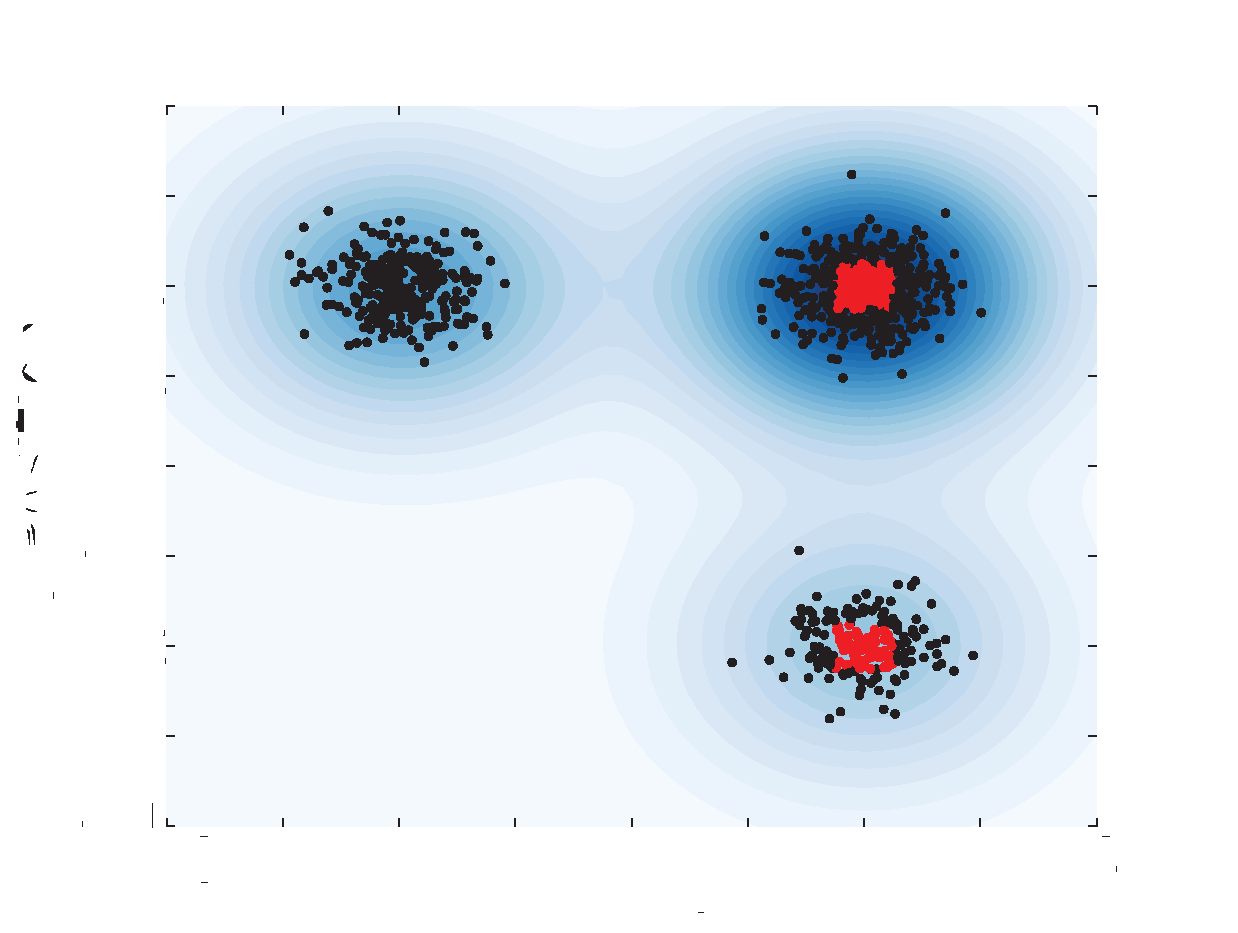
\includegraphics[width=5.5cm , height = 4.5cm]{figures/kde_gmm.eps}
\label{fig:subfigure1}}
\quad
\subfigure[One Class SVM]{%
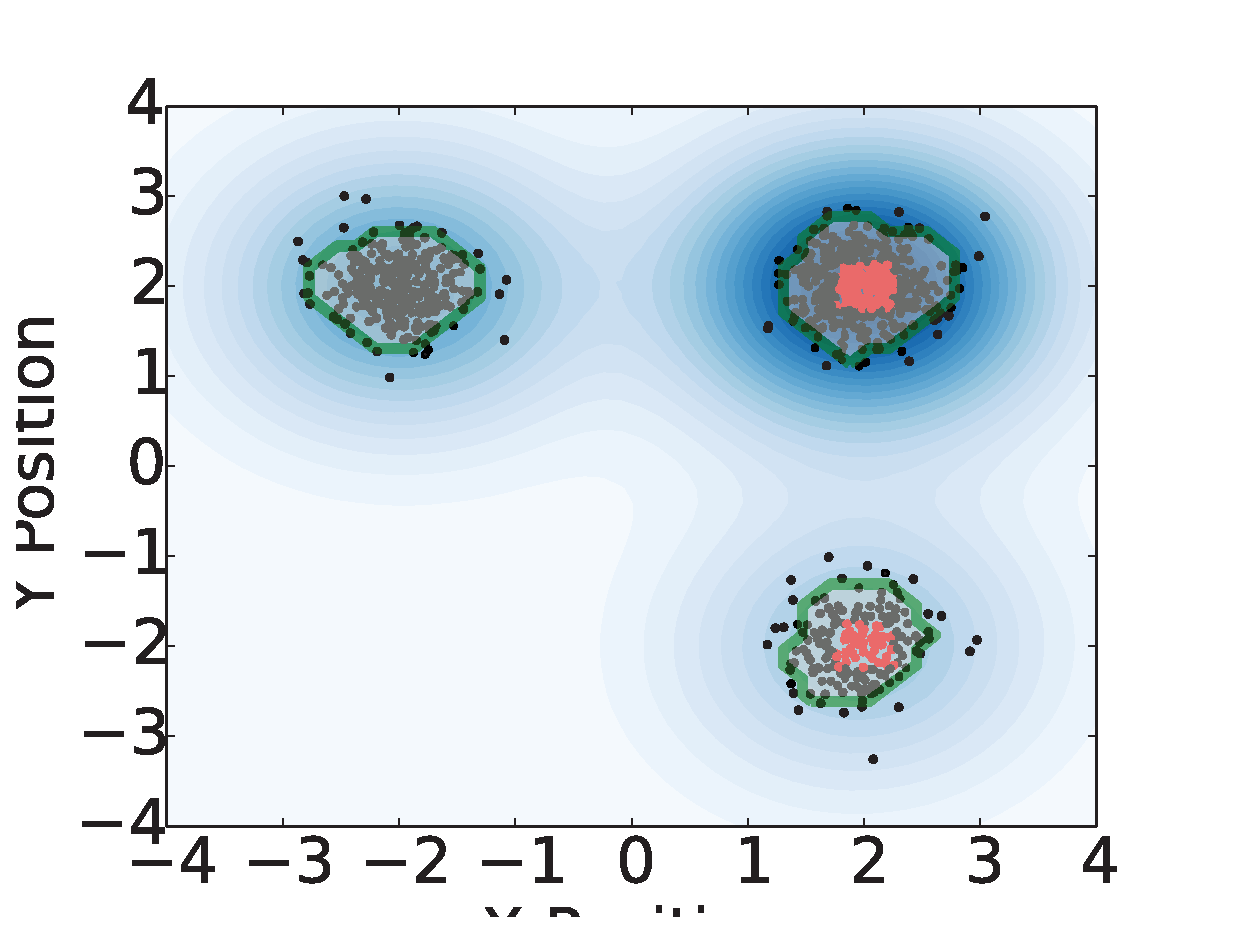
\includegraphics[width=5.5cm, height = 4.5cm]{figures/kde_gmm_ocm.eps}
\label{fig:subfigure2}}
\subfigure[Risk Sensitive One Class SVM]{%
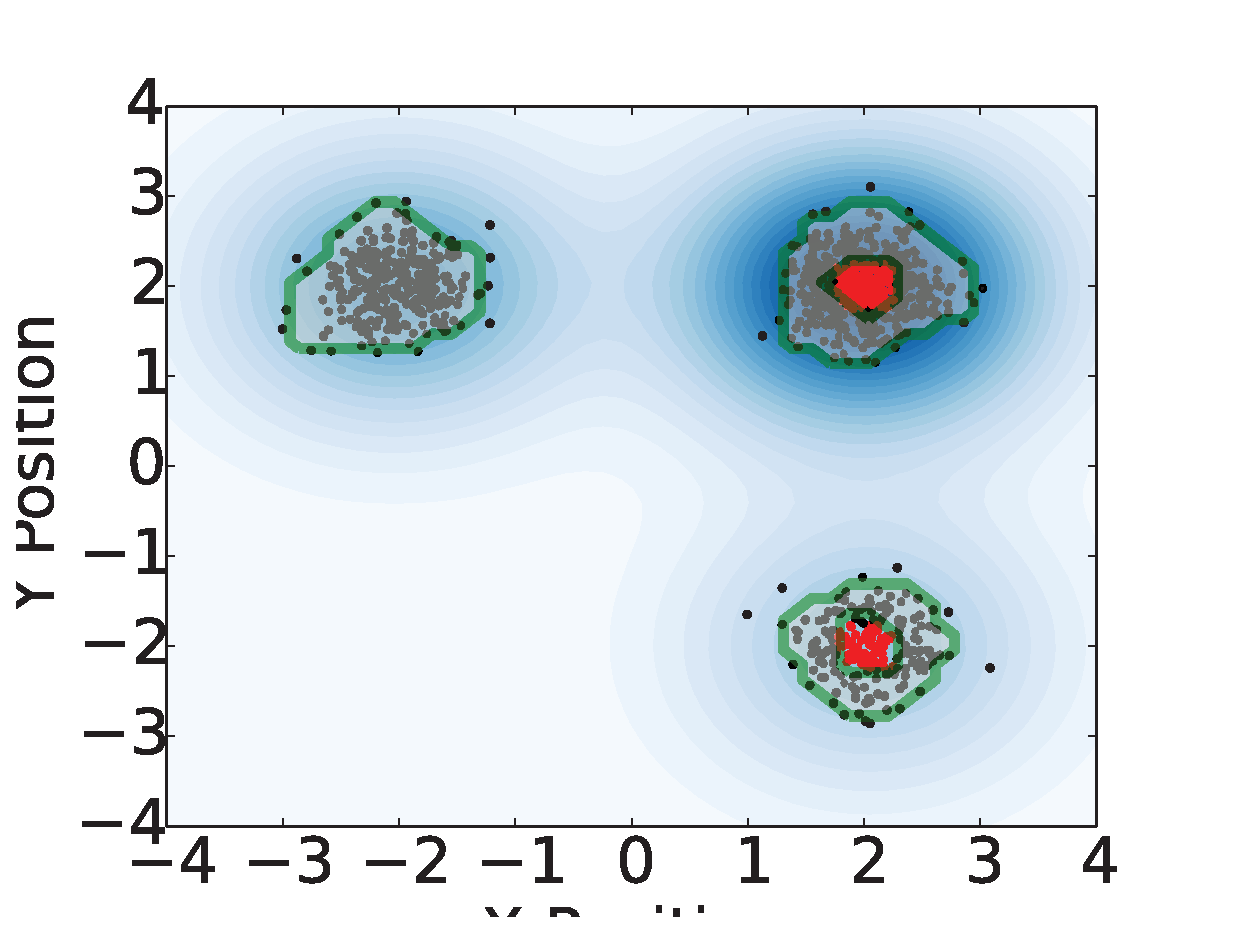
\includegraphics[width=5.5cm, height = 4.5cm]{figures/kde_gmm_mocm.eps}
\label{fig:subfigure3}}

\caption{We display synthetic data sampled from a Gaussian Mixture Model with three Gaussian components. In Fig.
\ref{fig:subfigure1}, the red points denote those that we assume a trained policy, $\pi_{theta}$ will mis-predict (i.e.
encounter large loss for). In Fig. \ref{fig:subfigure2}, the One Class SVM is fit to the data and tries to estimate the
areas of low risk (the light green region). While the densest area of data samples is enclosed, the standard One Class
svm is not able to incorporate information about samples on which our policy incurrs large loss. In Fig.
\ref{fig:subfigure3}, our modification - Risk Sensitive One Class SVM - is able to effectively remove the red points
with high loss from the region of low risk.}
\label{fig:support_example}
\end{figure*}

Let $\Phi:\mathcal{X}\to \mathcal{F}$ denote the feature map corresponding to our exponential kernel, mapping the
observation space $\mathcal{X}$ into a Hilbert space $(\mathcal{F}, \langle, \rangle)$ such that $k(\bx, \bx') = \langle
\Phi(\bx), \Phi(\bx')\rangle$.

The One Class SVM proposed by \cite{scholkopf2001estimating} determines a hyperplane in feature space $\mathcal{F}$
maximally separating the input data from the origin:
\vspace{-2ex}
\begin{align}\label{eq:primal_sup}
    \underset{w\in \mathcal{F}, \mathbf{\xi} \in \mathbb{R}, \rho \in \mathbb{R}}{\mbox{min}}\: \frac{1}{2}||w||^2+\frac{1}{vn} \sum^n_i \xi_i - \rho\\
\mbox{s.t} \: \langle w,\Phi(x_i) \rangle \geq \rho - \xi_i, \: \xi_i \geq 0 \notag.
\end{align}

Here, the parameter $\nu$ controls the penalty or `slack term' and asymptotically approaches $\gamma$ \cite{vert2006consistency}
in the quantile definition when bandwidths decay at appropriate rates as the number of samples increases. The decision
function, determining point membership in the approximate quantile levelset is given by

\vspace{-2ex}
\begin{align}\label{eq:decision_func}
g(x) = \mbox{sgn}(\langle w,\Phi(x) \rangle-\rho).
\end{align}

Where, for $x\in \mathcal{X}$, $g(x)=0$ if $x$ lies on the quantile levelset,
$g(x) = 1$ if $x$ is strictly in the interior of the quantile super-levelset and $g(x) = -1$ 
if $x$ lies strictly in the quantile sub-levelset. The dual form of the optimization yields a Quadratic Program 
that can be solved efficiently \cite{scholkopf2001estimating}. 

For training data in $\mathcal{X}$, we consider the quantile super-levelset for a user-defined threshold $\mu$ as a natural region within which
a trained policy $\pi_{\theta}$ can likely be learned since a sufficient data-density is available.
However, even when sufficient data is available, the associated control inputs may be inconsistent or noisy and a resulting policy
optimizing Eq. \ref{eq:super_objj} may still incur a large surrogate loss. To account for this, we propose a
modification to the One Class SVM:

\begin{align}
y_i = \left\{
     \begin{array}{lr}
         1 & : l(\pi_{\theta}(\bx_i),\bu_i)\le \varepsilon\\
         -1 & : l(\pi_{\theta}(\bx_i),\bu_i)>\varepsilon
     \end{array}
   \right.
\end{align}
Where, in the case when $l$ denotes discrete $0-1$ loss, we set $\varepsilon = 0$, while in the continuous $L_2$ loss
case, $\varepsilon$ is a user defined threshold specifying allowable surrogate loss.
We use $y_i$ to modify the One Class SVM optimization objective as follows: 

\vspace{-2ex}
\begin{align}\label{eq:primal_sup}
    \underset{w\in F, \mathbf{\xi} \in \mathbb{R}^l, \rho \in \mathbb{R}}{\mbox{min}}\: \frac{1}{2}||w||^2+\frac{1}{vn} \sum^n_i \xi_i - \rho\\
\mbox{s.t} \: y_i \langle w,\Phi(x_i)\rangle \geq \rho - \xi_i, \: \xi_i \geq 0 \label{eq:ineq}.
\end{align}

States that incur loss above the $\varepsilon$ threshold are then enforced to lie on the opposite side of the
hyper-plane separating the origin from the data in the feature space. Practically, this modification corresponds to
`carving out holes' in the estimated quantile super-levelset such that neighborhoods around states with $y_i=-1$ are
exluded from the super-levelset.

The dual formulation to the modified optimization problem, which is solved in practice, is 
\vspace{-2ex}
\begin{align}\label{eq:dual_sup}
\underset{\alpha_i\in \mathbb{R}}{\mbox{min}} \sum_i^n \sum_j^n \alpha_i\alpha_j y_i y_jk(\bx_i,\bx_j)\\
\mbox{s.t} \: 0 \leq \alpha \leq \frac{1}{\nu n} \:, \sum_i^n \alpha_i = 1.
\end{align}

Our corresponding decision function $g:\mathcal{X}\to \mathbb{R}$ is then derived in terms of the support vectors as $g(\bx) = \sum_i^n
\alpha_i y_i k(\bx_i,\bx) - \rho$. To compute the $\rho$ term, we leverage the fact that for an optimal solution the
inequalities in Eq. \ref{eq:ineq} are equal for any $\alpha_j$ such that $0 < \alpha_j < \frac{1}{\nu n}$. Therefore we
can compute $\rho$ as  $\rho = \sum_i^n y_i \alpha_i k(\bx_i,\bx_j)$ \cite{scholkopf2001estimating} {\color{blue} [-- F:
explain this more --]}.




\subsection{The \acro~algorithm}

Our proposed method trains a policy, $\pi_{\theta_k}$, but also estimates where the policy is likely to accurately
predict the supervisor's control, by means of the thresholded surrogate just discussed.  
% Too vague:
%In the statistics community, a known property is that estimators are function will likely mis-classify if they are evaluated at points not in the distribution sampled from.
%Techniques such as importance sampling use this results to train estimators on data drawn from a different distribution \cite{tokdar2010importance}.  
To reduce the burdon on the supervisor, we estimate the training data's quantile level-set for a user-defined threshold
$\nu$ and further modify the corresponding super-levelset estimate by excluding neighborhoods of states that incur a loss
above a threshold $\varepsilon$ chosen by the user.
The user then only provides control input demonstrations for states of trajectory roll-outs that lie outside the
resulting risk-aware quantile super-levelset and we terminate roll-outs that are at a task-specific threshold $r(\bx) = \sum_i^n
\alpha_i \bx_i k(\bx_i,\bx)-\rho>r_0$ away from the decision boundary $g$ corresponding to this modified super-levelset.

{\color{blue} [-- F: use formal algorithm and explain here instead --]} 
\subsubsection{Step 1}

Similar to DAgger, at iteration $k$, the algorithm estimates a policy, $\pi_{\theta_k}$ on the dataset $\mathcal{D}_k$
by solving the optimization problem in Eq. \ref{eq:super_objj}. We then estimate the quantile super-levelset of the
training data state-distribution solving the optimization for the modified One Class SVM using the dataset $\mathcal{D}_k$. 
This yields a decision boundary $g_k(\bx)$, where is $g(\bx)\ge 0$ if a state $\bx$ is to be considered of `low risk' and $-1$ otherwise. 
 
 
 \subsubsection{Step 2}
 In DAgger, the policy $\pi_{\theta_k}$ is rolled out for a fixed number of time steps, however this could lead to the
 robot entering pathological states that are risky. To prevent this, we terminate the rolled out policy if the risk, is
 above some threshold $r(\bx_t) > r_0$.  Furthermore, instead of providing control inputs for every state, the supervisor is only required to 
 provide demonstrations of control inputs for states for which $g(\bx)=-1$.  These demonstrations are then added to the
 dataset $\mathcal{D}_{k+1}$ and the algorithm returns to Step 1. 

We note that the choise of user-defined thresholds $\nu$, $\epsilon$, $r_0$ yield an implicit trade-off
between exploration and exploitation. For large quantile super-levelsets, the robot is confident and asks the
supervisor only rarely for demonstrations. Similarly, large $\varepsilon$ values allow the robot to be tolerant to
incorrectly trained policies with large surrogate loss, while large $r_0$ settings allow the robot to explore risky
areas and obtain more labels from the supervisor in those regions.


\section{Theoretical Analysis}
{\color{blue} [-- VERY ROUGH FROM HERE --]} 
\subsection{Convergence Rate}
{\color{blue} [-- F: Please discuss $\beta_i$ when introducing DAgger --]} 
The convergence rate of DAgger is dependent on the probability of the expert taking over at each iteration $\beta_i$
\cite{ross2010reduction}. For \acro, this corresponds to the probability of leaving the support or $p(g(\mathbf{x}) =
-1|\pi_{\theta_i})$ . The intuition is that the larger the level set parameter $\nu$ is the lower the probability of
leaving is and thus we obtain faster convergence rates, but potentially need to apply risky roll-outs. We are not sure if a formal proof 
will be possible. However, we can experimentally demonstrate this. 


\section{Experiments}
\subsection{Driving Example}
A common benchmark in Reinforcement Learning is that of a car driving around a track while avoiding collisions with
other cars \cite{argall2009survey}. We implemented a car simulator where the car must stay on a rectangular track and
avoid autonomously controlled cars that drive on the same track. If the car accidentally leaves the track, it is placed
back on the center of the track at a nearby position. The car's control input space is  $\mathcal{U} = \lbrace -15^\circ, 0, 15^\circ \rbrace$
instantly changing the angle of the car that drives at a unit speed. The internal state space of the car is given by the
xy-coordinates and the angle it is facing. In our experiments, the supervisor is provided by an algorithm that uses
state space search through the driving simulator to plan the next control {\color{blue} [-- F: be more precise --]}.

The supervisor drives around the track twice. We collect raw images of the simulation from a 2D bird's eye view
and use Gaussian Pyramids to down-sample the images to $125 \times 125$ RGB pixels and then extract Histogram of
Oriented Gradients (HOG) features using OpenCV. These histograms serve as the \emph{observable state space}
$\mathcal{X}$. For both DAgger and \acro, we use a Linear Support Vector Machine (SVM) to parameterize allowable
policies $\pi_{\theta}$, with $\gamma=0.01$ as a regularization term on the slack variables, which was set via cross
validation on the initial training examples. For the optimization of Eq. \ref{eq:dual_sup} in \acro, we used an
exponential kernel with a bandwidth of $\lambda=0.01$ and $\nu = 0.95$ to account for $95\%$ of the training distribution. 
{\color{blue} [-- F: what about $r_0$? --]}

We compare the policy's performance in terms of minimization of an underlying cost function $c(\bx,\bu)$, which is
defined to be total number of times the car left the track or collided with the other cars on the track. We compare the
cost to the number of control input demonstrations queried from the supervisor. Initial results over 1 level shown in Fig.  suggest an $75\%$ reduction in the number of queries needed for SHEATH compared to DAgger. 

\begin{figure}[t!]
\centering
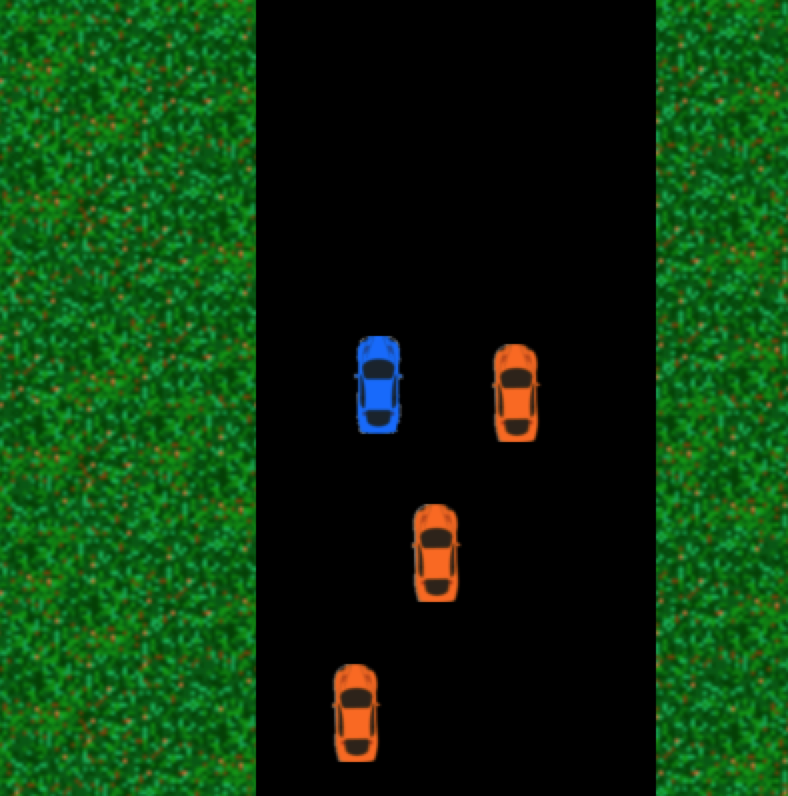
\includegraphics[width=6cm, height=6cm]{figures/race_car_track_example.png}
\caption{ An example image from the racing simulator. The car has to drive around a rectangular track and avoid other
cars. The supervisor drives around the track three times and HOG features are extracted from the images to represent
observable states.  }

\vspace*{-10pt}
\label{fig:race_car}
\end{figure}


\begin{figure}[t!]
\centering
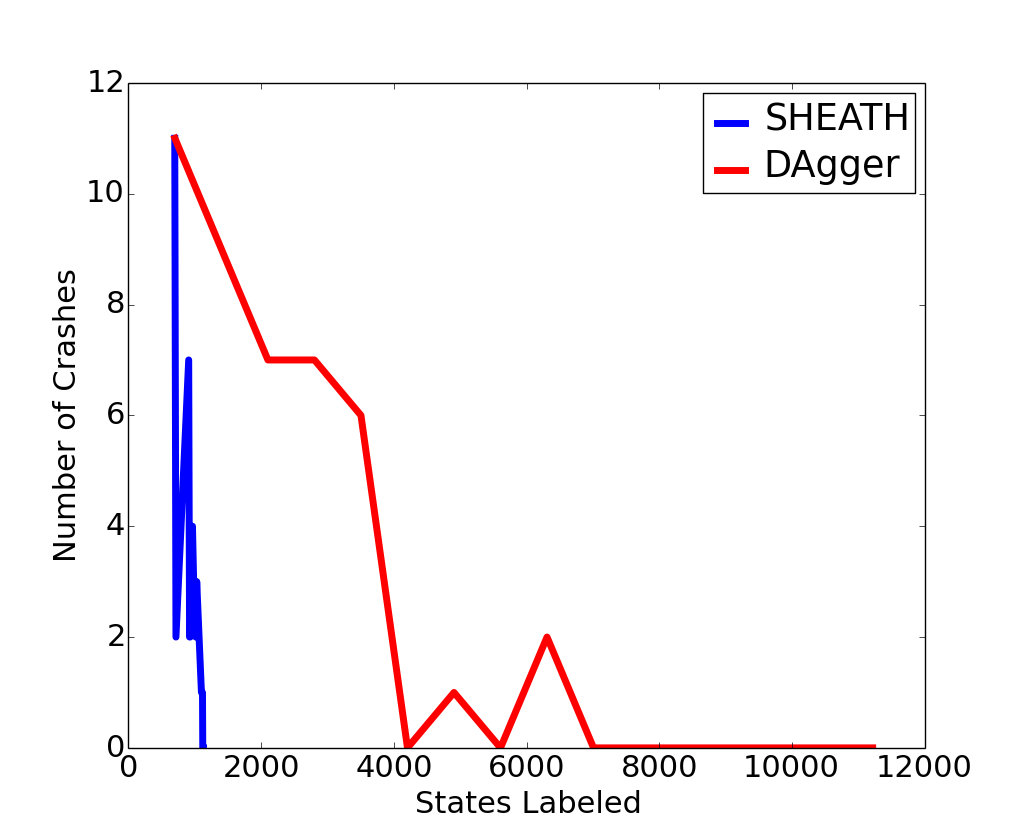
\includegraphics[width=8cm, height=6cm]{figures/dagger_sheath_no_cars.png}
\caption{ We compare performance in terms of optimization of the underlying cost function $c(\bx,\bu)$, which is given
    by the number of times the car left the track or collided with the other cars on the track. Initial results averaged
    over 1 level suggest a $75\%$ reduction in the number of queries needed for \acro~compared to DAgger.}

\vspace*{-10pt}
\label{fig:car_cost}
\end{figure}


\subsection{Super Mario Bros}
Super Mario Bros. is a platform video game where the character, Mario, must move across each level by avoiding being hit by enemies and falling into gaps, and before running out of time. We used the simulator from a recent Mario Bros. AI competition which can randomly generate stages of varying difficulty (more difficult gaps and types of enemies) \cite{marioAI}. Our goal is to train the computer to play the game based on current game features as input. Our expert is a near optimal $A^*$ search algorithm that plans ahead using the game simulator. 
The set of allowable control inputs $\mathcal{U}$ consists of 4 binary variables indicating which subset of buttons we
should press in $\lbrace \mbox{left},\mbox{right},\mbox{jump},\mbox{speed} \rbrace$. For both DAgger and \acro~, we use
a Linear Support Vector Machine (SVM) as the policy representation, with the regularization on the slack variable given
by $\gamma=0.01$, which was set via cross validation on the initial training examples from our expert. We initialized
both Dagger and \acro~with two expert demonstrations for each level. For the optimization of Eq. \ref{eq:dual_sup} in
\acro~, we used an exponenital kernel with a bandwidth of $c=0.01$ and $\nu = 0.95$ to account for a $95\%$ quantile.

\begin{figure}[t!]
\centering
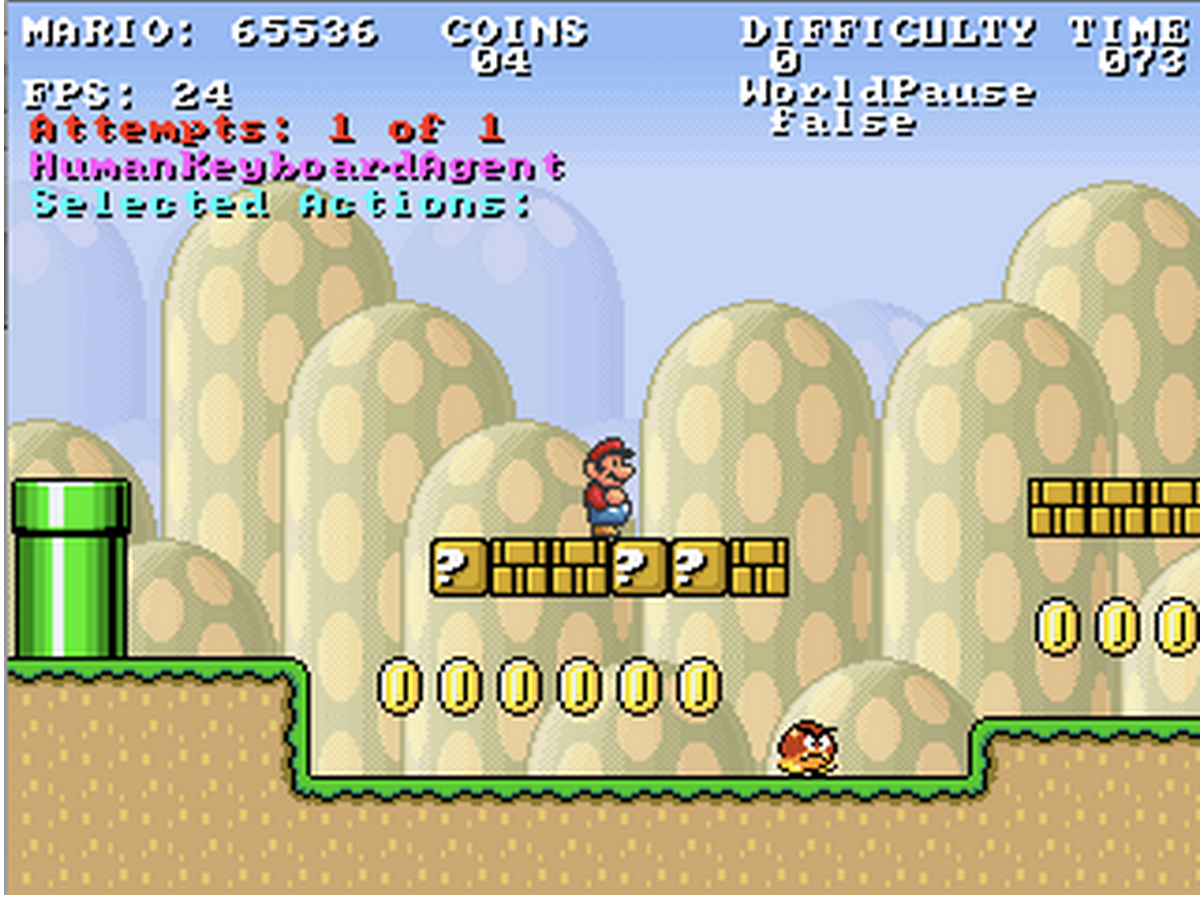
\includegraphics[width = 6cm ]{figures/mario.png}
\caption{ An example image from the Mario AI simulator. Mario faces many challenges to reach an end of a level, such as gaps, jumps and enemies.  }

\vspace*{-10pt}
\label{fig:dis_traveled}
\end{figure}



\begin{figure}[ht]
\centering

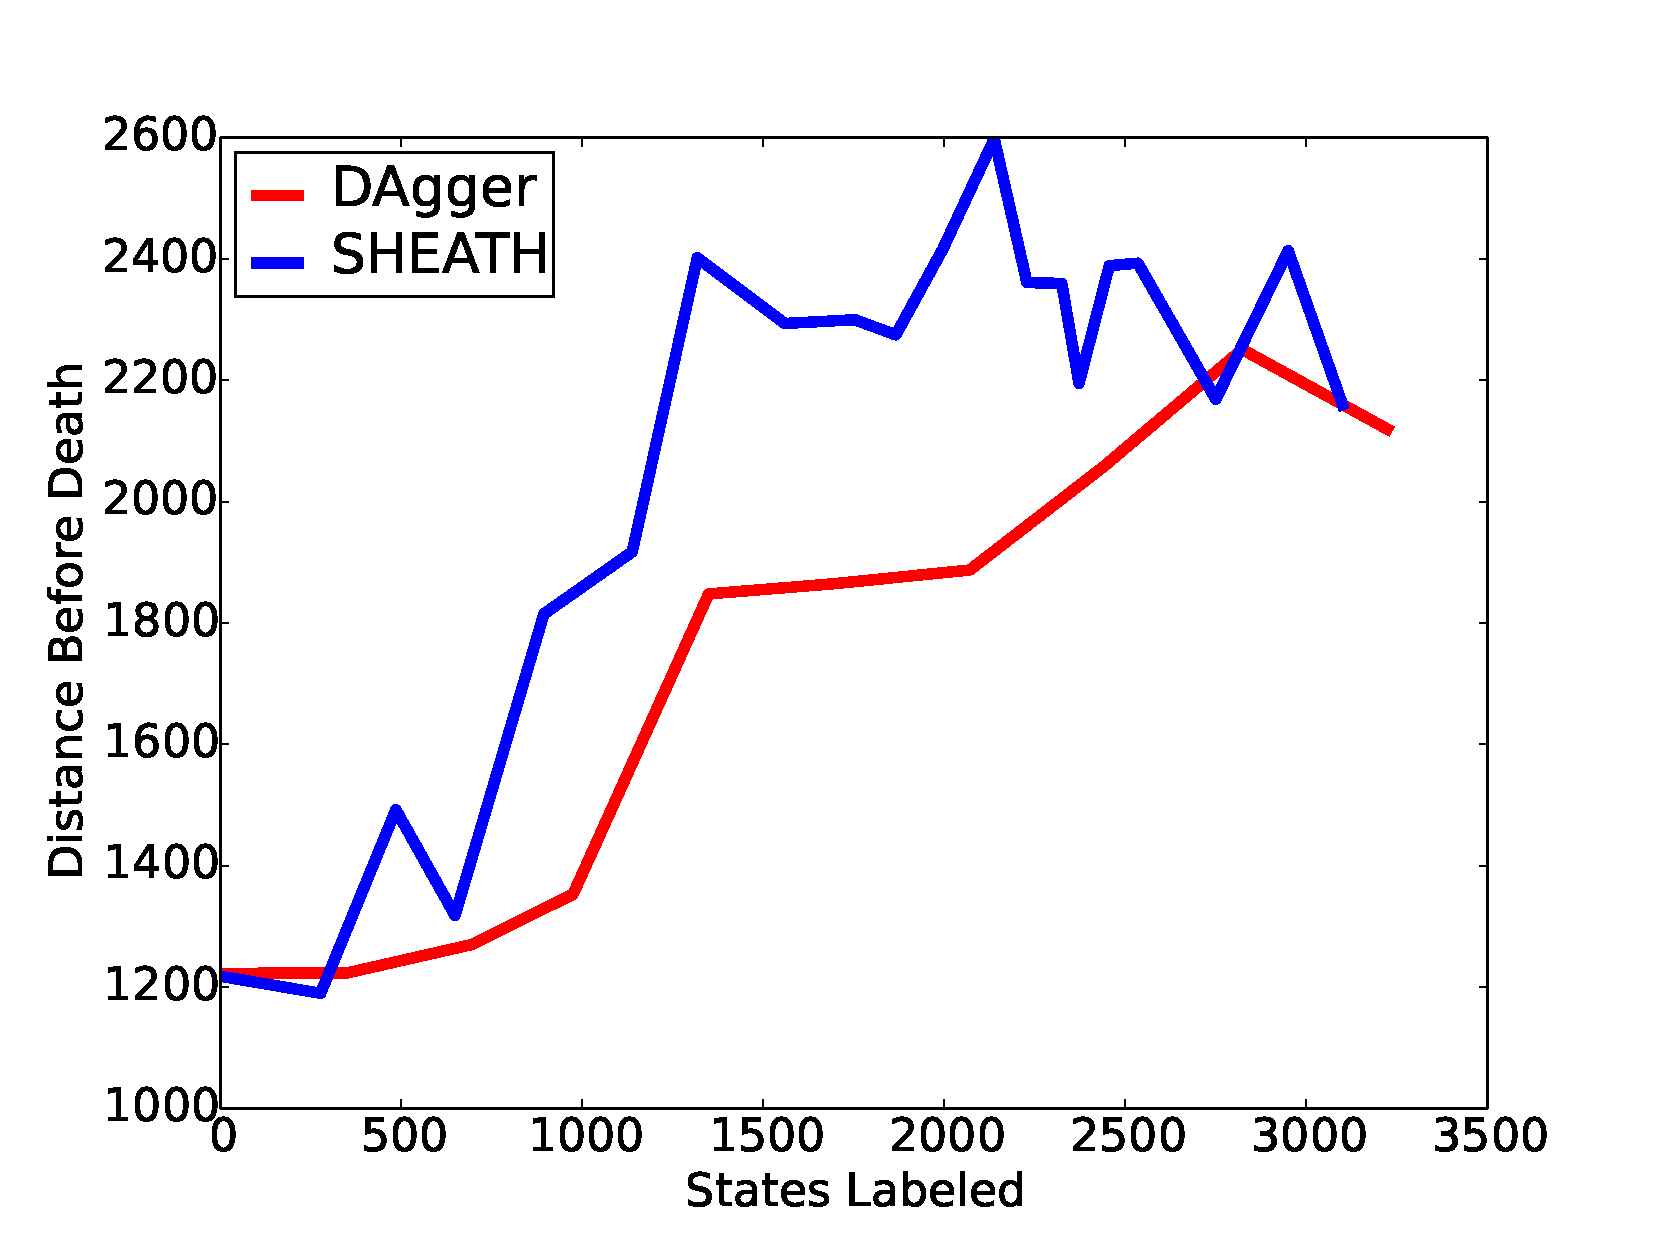
\includegraphics[width=8cm, height = 4.5cm]{figures/dagger_sheath_mario.eps}


\caption{We compare performance in terms of average distance traveled by Mario per stage before dying, running out of
time or completing the stage, on randomly generated stages of difficulty 1 with a time limit of 35s to complete the
stage.  Stages of difficulty 1 are fairly easy for an average human player but contain most types of enemies and gaps,
except with fewer enemies and gaps than stages of harder difficulties. We compare performance of our method and DAgger.
In Fig. \ref{fig:mario_results}, we report the performance of distance traveled vs. the number of labels provided by the
supervisor. Initial results, averaged over 20 levels, suggest \acro~ was able to reach DAgger's peak performance of a
distance around 2200 with only 1200 labels, while DAgger required 2800. {\color{blue} [-- very preliminary --]}}
\label{fig:mario_results}
\end{figure}


\subsection{Other Experiments}
{\color{blue} [-- maybe a controller for a robot arm --]}

\section{Discussion and Future Work}


\bibliographystyle{IEEEtranS}
\bibliography{references}



\end{document}
